
\begin{table*}
\centering \caption{We varied $T$, the expected number of topical relevance (rows), and the mean $\mu$ of Gaussian distribution used to generate understandability labels (columns). 
    A smaller $\mu$ means that easier to read documents are retrieved.
    We showed the average and standard deviation of each experiment. All numbers were multiplied by 100. }
\label{tab:simulations} \resizebox{1.\textwidth}{!}{ %
\begin{tabular}{cllllllllllll}
\toprule 
\multirow{2}{*}{$T$}  & \multicolumn{4}{c}{\textbf{Understandability $\mathcal{N}$(50,40)}} & \multicolumn{4}{c}{\textbf{Understandability $\mathcal{N}$(40,40)}} & \multicolumn{4}{c}{\textbf{Understandability $\mathcal{N}$(30,40)}}\tabularnewline
\cmidrule{2-13}
 & RBP  & uRBP  & $RBP_{u}$  & $H_{RBP}$  & RBP  & uRBP  & $RBP_{u}$  & $H_{RBP}$  & RBP  & uRBP  & $RBP_{u}$  & $H_{RBP}$ \tabularnewline
\midrule 
0.3 & 28$\pm$1 & 14$\pm$1 & 41$\pm$1 & 30$\pm$1 & 28$\pm$1 & 16$\pm$1 & 50$\pm$1 & 33$\pm$1 & 28$\pm$1 & 19$\pm$1 & 59$\pm$2 & 35$\pm$1\tabularnewline
0.4 & 38$\pm$2 & 19$\pm$1 & 41$\pm$1 & 36$\pm$1 & 38$\pm$2 & 21$\pm$1 & 50$\pm$1 & 39$\pm$1 & 38$\pm$2 & 25$\pm$1 & 60$\pm$1 & 43$\pm$1\tabularnewline
0.5 & 47$\pm$1 & 24$\pm$1 & 41$\pm$1 & 40$\pm$1 & 47$\pm$1 & 26$\pm$1 & 49$\pm$1 & 45$\pm$1 & {\cellcolor{yellow!25}} 47$\pm$1 & {\cellcolor{yellow!25}} 30$\pm$1 & {\cellcolor{yellow!25}} 60$\pm$1 & {\cellcolor{yellow!25}} 49$\pm$1\tabularnewline
0.6 & 56$\pm$1 & 28$\pm$1 & 41$\pm$1 & 44$\pm$1 & {\cellcolor{blue!25}}56$\pm$1 & {\cellcolor{blue!25}}32$\pm$1 &  {\cellcolor{blue!25}}49$\pm$2 & {\cellcolor{blue!25}}49$\pm$1 & 56$\pm$1 & 37$\pm$1 & 60$\pm$1 & 55$\pm$1\tabularnewline
0.7 & 65$\pm$1 & 33$\pm$1 & 42$\pm$1 & 48$\pm$1 & 65$\pm$1 & 37$\pm$1 & 49$\pm$1 & 53$\pm$1 & 65$\pm$1 & 42$\pm$1 & 60$\pm$1 & 60$\pm$1\tabularnewline
\bottomrule
\end{tabular}} 
\end{table*}




\section{Comparing frameworks Through System Simulations}
\label{sec:simulations}

%While Section~\ref{sec:understandability_metrics} revised uRBP, Zuccon's modification of the gain-discount framework to incorporate understandability along with topicality in one single formula,
%Section~\ref{sec:extension} proposed an alternative approach which calculates an score for each dimension first and then combine these scores into a unique value with an harmonic mean.
%In this section, we aim to evaluate uRBP and $H_{RBP}$, our proposed alternative, comparing each other with simulations.
%\mytodo{Start by a reason to use simulations in this work}

To understand the behaviour of UBIRE and H when facing different IR systems, we first employed synthetic systems so as to have a fine-grained control over our experiments. This allowed to know a-priori what has changed between two system instances and study the effect these changes had on evaluation. In our experiments, along with topicality, we considered understandability, leaving the (trivial) extension to other dimensions to later work. 
In the following simulations we controlled the amount of topical documents and understandable documents retrieved. We did so by following this two-phase procedure:
%\mytodo{Find some other paper that made their evaluation with simulated systems}.


%The aim of this section is to understand the behaviour of each evaluation framework when facing different types of Information Retrieval systems.
%In order to have a fine-grained control over our experiments, we employed synthetic/simulated systems.
%This way, we know exactly what to expect from each system and evaluation metric before calculating any score.


%Through the expected results of the simulated systems, we demonstrate how the proposed two-step framework, $H$ (Section~\ref{sec:extension}), fixes the main drawback found in Zuccon's modification of the gain-discount framework (Section~\ref{sec:understandability_metrics}). 
%
%Without loss of generality, we set our further experiments in the same context as UBIRE was proposed: to evaluate both topicality and understandability of documents in the context of consumer health search. This decision helps the flow of this paper, but by no means these frameworks are limited to evaluate this specific dimensions. 

%In our further experiments, we have full control over both topical and understandability relevance of documents. 
%The behaviour of the proposed evaluation metrics is investigated when we slightly increase/decrease the amount of topically relevant documents or when we increase/decrease the expected reading difficult of the retrieved documents. 
%For that, we generated simulated runs following the this two-phases procedure:

\begin{enumerate}
\item \textbf{Topicality Phase:} we exclusively controlled the amount of topical documents in a simulated run using a random variable $T$, $0 \le T \le 1$. 
We constructed a synthetic run by drawing a real number $N_i$, $0 \le N_i \le 1$, for each position $i$ in a ranking. If $N_i \le T$, we marked the document at position $i$ as relevant, otherwise, we marked it as not relevant. It is expected that a run generated with $T=0.1$ has 10\% of the documents assessed as relevant (90\% as non-relevant), while a run with $T=0.5$ has as many relevant as non-relevant documents. 

\item \textbf{Understandability Phase:}  we controlled the level of understandability of the documents in a synthetic run. In order to create and control the randomness of our synthetic systems, we generated understandability labels using a Gaussian distribution with pre-defined mean $\mu$ and variance $\sigma$. 
As previously done in consumer health search collections~\cite{clefIR16,clefIR17}, we forced the understandability labels to be in the interval $[0,100]$. 
We fixed a relatively large variance, $\sigma=40$, to mimic results of previous collections in which the understandability labels had a large variance \cite{clefIR16}, and we varied the mean $\mu$ of the Gaussian from 0 to 100. Figure~\ref{fig:gaussians} shows the expected label distribution for $\mu=20, 50, 80$, i.e., $\mathcal{N}(20, 40)$, $\mathcal{N}(50, 80)$ and $\mathcal{N}(80, 40)$.
In Figure~\ref{fig:gaussians} we also included the threshold U used to compute $RBP_u$ (Section~\ref{sec:extension}).
\end{enumerate}

We executed these two phases in succession. In total, we generated 1,000 runs for each topical level (topicality phase) and $\mu$ value (understandability phase). 


%\begin{enumerate}
%\item \textbf{Topicality Phase:} In this phase, we exclusively control the amount of topical relevant documents in a simulated run. That is done with a simple random variable $T$, $0 \le T \le 1$. 
%We constructed a simulated run by drawing a real number $N$, $0 \le N \le 1$, for each position $i$ in a ranking. If $N \le T$, we mark the document at position $i$ as relevant, otherwise, we mark that document as not relevant. It is expected that a run generated with $T=0.1$ would have 10\% of the documents assessed as relevant and 90\% as non-relevant, while a run with $T=0.5$ will have as many relevant as non-relevant documents. 
%
%\item \textbf{Understandability Phase:}  Once the previous phase is done, we start this one. Here, we control the level of understandability of the results. In order to create and control the randomness of our simulated systems, we generate understandability labels with a Gaussian distribution with pre-defined mean $\mu$ and variance $\sigma$. 
%As previously done in consumer health search collections~\cite{clefIR16,clefIR17}, we force the understandability labels generated to be in the interval from 0 to 100. 
%We fixed a relatively large variance, $\sigma=40$, to mimic results of previous collections in which the understandability labels have a large variance \cite{clefIR16}, and we vary the mean $\mu$ of the Gaussian from 0 to 100. Figure~\ref{fig:gaussians} shows the expected label distribution for $\mu=20, 50, 80$, i.e., $\mathcal{N}(20, 40)$, $\mathcal{N}(50, 80)$ and $\mathcal{N}(80, 40)$.
%In Figure~\ref{fig:gaussians} we also include the threshold U used to compute $RBP_u$ (Section~\ref{sec:extension}).
%
%\end{enumerate}

\begin{figure}[t!]
  \centering
   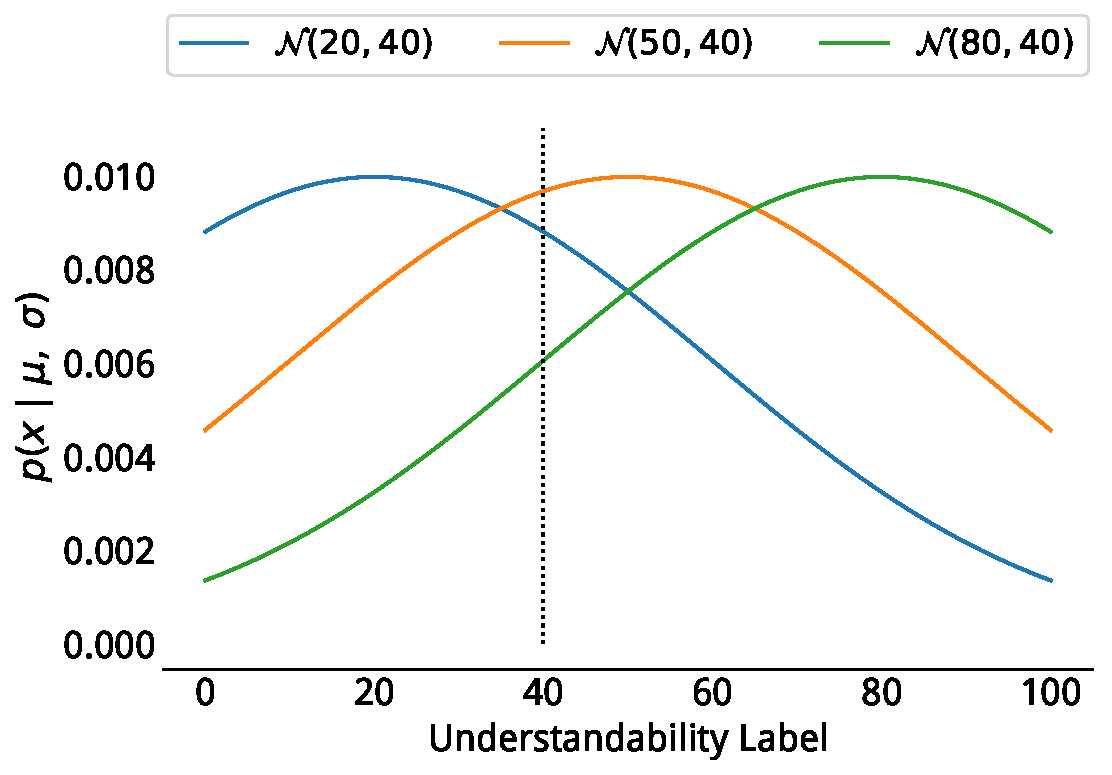
\includegraphics[width=0.30\textwidth]{figs/gaussians}
    \vspace{-.2cm}
    \caption{Gaussian distribution for different $\mu$: higher $\mu$ generates higher understandability labels (harder documents were retrieved). Here, only documents with understandability lower than 40 are considered easy-to-understand. (Understandability threshold shown as dotted line). \vspace{-16pt}}
  \label{fig:gaussians}
\end{figure}


We calculated $uRBP$ (using UBIRE) and $H_{RBP}$ for each synthetic system.
The average result of the synthetic runs is shown in Table~\ref{tab:simulations}. Each row shows the results of simulations with different values for $T$, i.e., different expected number of topical documents retrieved.
We varied $\mu$ which was used to create the understandability labels, and show the results for $\mu = 50, 40, 30$.
A smaller $\mu$ means that more understandable documents were retrieved. The results shows that as the expected number of topical documents ($T$) increases, $RBP$ increases. Likewise, $uRBP$ increases, as it is bounded by topical relevance.
In turn, increasing $T$ has no effect on $RBP_u$, but increases $H_{RBP}$, as it is also directly dependant on $RBP$. When the number of understandable documents retrieved is increased (i.e., $\mu$ decreased ), $RBP$ stays constant, as it does not measure how understandable documents are.
In turn, $uRBP$, $RBP_u$ and $H_{RBP}$ increase. 
Those are the expected behaviour of the considered measures. % aforementioned metrics and only shows that our simulated runs produce sane results.

We further focused our attention to the results of specific experiments highlighted in blue and yellow in Table~\ref{tab:simulations}. These cases simulated an initial system S1 that exhibited the results in blue (condition $T=0.6$ and $\mathcal{N}(40,40)$) being modified to improve the understandability of retrieved documents ($\mathcal{N}(30,40)$) at the expenses of topicality ($T=0.5$), producing a new system S2. The effectiveness of S2 is highlighted in yellow. 

If $RBP$ and $uRBP$ were used to decide whether S2 should be preferred over the initial system S1, then S2 would be discarded and S1 preferred, as S2 produced a $18\%$ reduction in $RBP$ and a $13\%$ reduction in $uRBP$. With these results, an IR researcher would conclude that the modifications in S2 did not pay off.

If $H_{RBP}$ was used instead, the IR researcher would have been able to gain more insights about system effectiveness and the trade-off between understandability and topicality. To use $H_{RBP}$, $RBP_t$ ($=RBP$) and $RBP_u$ needed to be computed. Between S1 and S2, there was a decrease in $RBP_t$ of $18\%$; but conversely $RBP_u$ increased of $24\%$: this clearly allows to gauge the trade-off between topicality and understandability. 

When $RBP$ and $uRBP$ were combined within $H_{RBP}$, if both dimensions were given equal weight, then systems S1 and S2 obtained the same $H_{RBP}$. Note that $H$ can be adapted to specific circumstances: if topicality was more important than understandability, then the weights of each dimension would have been changed accordingly in the harmonic mean computation. 




%
%
%The trick part that we aim to show with these experiments is illustrated by the cells colored in blue and yellow in Table~\ref{tab:simulations}.
%We modeling and experimenting with a retrieval system, a modification that aims to increase the understandability of the documents retrieved by the system might hurt the topical relevance of the documents retrieved by the system.
%This situation could be translated in an initial system with results shown in blue in Table~\ref{tab:simulations} (i.e., $T=0.6$ and $\mathcal{N}(40,40)$) 
%being modified into the system with results shown in yellow ($T=0.5$ and $\mathcal{N}(30,40)$).
%
%If the person doing the system modification considers only the $RBP$ and the $uRBP$, she would definitely discard the new systems (marked in yellow in Table~\ref{tab:simulations}) as both $RBP$ and $uRBP$ decreased ($RBP$ decreased from 56 to 47 and $uRBP$ decreases from 32 to 30). Based only on $RBP$ and $uRBP$ from UBIRE framework, it is not possible to notice the gains in the understandability dimension.
%
%However, when separately measuring $RBP_t$ (which is the same as $RBP$) and $RBP_u$, we can understand better what is happening with each dimension: $RBP_t$ decreases from 56 to 47, but $RBP_u$ increases from 49 to 60, i.e., the trade-off between the two dimensions is clearly shown.
%Finally, $H_{RBP}$, which is instantiated to give the same importance to both dimensions, shows that, although very different, both system are equivalent. 
%In a real system, if document topicality is more important than document understandability, the weights of each dimension can be tweaked in the harmonic mean formula, exactly as precision and recall are balanced in the $F$ formula.

 

%%%%%%%%%%%%%%%%%%%%%%%%%%%%%%%%%%%%%%%%%%%%%%%%%%%%%%%%%%%%%%%%%%%%%%%%%%%%%%%%%%%%%%%%%%%%%%%%%%%%%%%%%%%%%%%%%%%%%%%%%%%%%%%%
%%%%%%%%%%%%%%%%%%%%%%%%%%%%%%%%%%%%%%%%%%%%%%%%%%%%%%%%%%%%%%%%%%%%%%%%%%%%%%%%%%%%%%%%%%%%%%%%%%%%%%%%%%%%%%%%%%%%%%%%%%%%%%%%
%%%%%%%%%%%%%%%%%%%%%%%%%%%%%%%%%%%%%%%%%%%%%%%%%%%%%%%%%%%%%%%%%%%%%%%%%%%%%%%%%%%%%%%%%%%%%%%%%%%%%%%%%%%%%%%%%%%%%%%%%%%%%%%%
%%%%%%%%%%%%%%%%%%%%%%%%%%%%%%%%%%%%%%%%%%%%%%%%%%%%%%%%%%%%%%%%%%%%%%%%%%%%%%%%%%%%%%%%%%%%%%%%%%%%%%%%%%%%%%%%%%%%%%%%%%%%%%%%

